

\documentclass[14pt]{scrartcl} % Font size
\usepackage{xcolor}
\usepackage{multirow}
\usepackage{multicol}
\usepackage{colortbl}
%%%%%%%%%%%%%%%%%%%%%%%%%%%%%%%%%%%%%%%%%
% Wenneker Assignment
% Structure Specification File
% Version 2.0 (12/1/2019)
%
% This template originates from:
% http://www.LaTeXTemplates.com
%
% Authors:
% Vel (vel@LaTeXTemplates.com)
% Frits Wenneker
%
% License:
% CC BY-NC-SA 3.0 (http://creativecommons.org/licenses/by-nc-sa/3.0/)
% 
%%%%%%%%%%%%%%%%%%%%%%%%%%%%%%%%%%%%%%%%%

%----------------------------------------------------------------------------------------
%	PACKAGES AND OTHER DOCUMENT CONFIGURATIONS
%----------------------------------------------------------------------------------------

\usepackage{amsmath, amsfonts, amsthm} % Math packages

\usepackage{listings} % Code listings, with syntax highlighting

\usepackage[english]{babel} % English language hyphenation

\usepackage{graphicx} % Required for inserting images
\graphicspath{{Figures/}{./}} % Specifies where to look for included images (trailing slash required)

\usepackage{booktabs} % Required for better horizontal rules in tables

\numberwithin{equation}{section} % Number equations within sections (i.e. 1.1, 1.2, 2.1, 2.2 instead of 1, 2, 3, 4)
\numberwithin{figure}{section} % Number figures within sections (i.e. 1.1, 1.2, 2.1, 2.2 instead of 1, 2, 3, 4)
\numberwithin{table}{section} % Number tables within sections (i.e. 1.1, 1.2, 2.1, 2.2 instead of 1, 2, 3, 4)

\setlength\parindent{0pt} % Removes all indentation from paragraphs

\usepackage{enumitem} % Required for list customisation
\usepackage{caption}
\usepackage{subcaption}
\setlist{noitemsep} % No spacing between list items

%----------------------------------------------------------------------------------------
%	DOCUMENT MARGINS
%----------------------------------------------------------------------------------------

\usepackage{geometry} % Required for adjusting page dimensions and margins

\geometry{
	paper=a4paper, % Paper size, change to letterpaper for US letter size
	top=2.5cm, % Top margin
	bottom=3cm, % Bottom margin
	left=3cm, % Left margin
	right=3cm, % Right margin
	headheight=0.75cm, % Header height
	footskip=1.5cm, % Space from the bottom margin to the baseline of the footer
	headsep=0.75cm, % Space from the top margin to the baseline of the header
	%showframe, % Uncomment to show how the type block is set on the page
}

%----------------------------------------------------------------------------------------
%	FONTS
%----------------------------------------------------------------------------------------

\usepackage[utf8]{inputenc} % Required for inputting international characters
\usepackage[T1]{fontenc} % Use 8-bit encoding

\usepackage{fourier} % Use the Adobe Utopia font for the document

%----------------------------------------------------------------------------------------
%	SECTION TITLES
%----------------------------------------------------------------------------------------

\usepackage{sectsty} % Allows customising section commands

\sectionfont{\vspace{6pt}\centering\normalfont\scshape} % \section{} styling
\subsectionfont{\normalfont\bfseries} % \subsection{} styling
\subsubsectionfont{\normalfont\itshape} % \subsubsection{} styling
\paragraphfont{\normalfont\scshape} % \paragraph{} styling

%----------------------------------------------------------------------------------------
%	HEADERS AND FOOTERS
%----------------------------------------------------------------------------------------

\usepackage{scrlayer-scrpage} % Required for customising headers and footers

\ohead*{} % Right header
\ihead*{} % Left header
\chead*{} % Centre header

\ofoot*{} % Right footer
\ifoot*{} % Left footer
\cfoot*{\pagemark} % Centre footer


\usepackage{xcolor}
\usepackage{multirow}
\usepackage{multicol}
\usepackage{colortbl}

\usepackage{algpseudocode} % Include the file specifying the document structure and custom commands

%----------------------------------------------------------------------------------------
%	TITLE SECTION
%----------------------------------------------------------------------------------------

\title{	
	\normalfont\normalsize
	\textsc{Department of Computer Science and Engineering, BUET}\\ % Your university, school and/or department name(s)
	\vspace{25pt} % Whitespace
	\rule{\linewidth}{0.5pt}\\ % Thin top horizontal rule
	\vspace{20pt} % Whitespace
	{\huge NS2 offline-1 Report}\\ % The assignment title
	\vspace{12pt} % Whitespace
	\rule{\linewidth}{2pt}\\ % Thick bottom horizontal rule
	\vspace{12pt} % Whitespace
}

\author{\LARGE Ruhul Azgor \\ 1805091} % Your name

\date{\normalsize\today} % Today's date (\today) or a custom date

\begin{document}

\maketitle % Print the title

%----------------------------------------------------------------------------------------
%	FIGURE EXAMPLE
%----------------------------------------------------------------------------------------

\section*{}

\begin{figure}[h] % [h] forces the figure to be output where it is defined in the code (it suppresses floating)
	\centering
	
\includegraphics[width=0.5\columnwidth]{Figures/BUET_LOGO.svg.png} % Example image
	 
\end{figure}

%------------------------------------------------
\pagebreak
%----------------------------------------------------------------------------------------
%	TEXT EXAMPLE
%----------------------------------------------------------------------------------------
\section{Description}
\subsection{MAC type (IEEE 802.11) }
\textbf{IEEE 802.11} is a set of standards for wireless local area network (WLAN) computer communication, developed and maintained by the Institute of Electrical and Electronics Engineers (IEEE). It specifies the physical layer and the media access control (MAC) of wireless LANs. The standard is used for wireless networks that operate in the 2.4 GHz, 5 GHz, and 6 GHz frequency bands. There are many variations of the 802.11 standard, including 802.11a, 802.11b, 802.11g, 802.11n, and 802.11ac. Each of these variations provides different capabilities and data transfer speeds. For example, 802.11a provides higher data transfer rates and operates in the 5GHz band while 802.11b operates in 2.4GHz band and has lower data transfer rates.

\subsection{Routing Protocol (AODV)}
\textbf{AODV} (Ad-hoc On-Demand Distance Vector) is a routing protocol for mobile ad-hoc networks (MANETs). It is a reactive protocol, meaning that it only establishes a route between two nodes when it is required. AODV operates on a demand-driven approach, where a route is established only when a node requests it.

AODV uses a routing table to keep track of the routes to other nodes in the network. Each entry in the table contains the destination node's address, the next hop to reach the destination, and a sequence number that is used to ensure that the route is up-to-date. When a node wants to send a packet to another node, it checks its routing table for a valid route. If a route is not found, the node initiates a route discovery process by broadcasting a RREQ (Route Request) packet.

When a node receives a RREQ packet, it checks if it has a route to the destination node. If it does, it sends a RREP (Route Reply) packet back to the source node along the reverse path. If it doesn't, it rebroadcasts the RREQ packet. When the destination node receives the RREQ packet, it sends a RREP packet back to the source node, and the route is established.
AODV is a simple and efficient routing protocol, but it is not suitable for large-scale networks because it can result in high control overhead and long route discovery latency. It is useful for small-scale networks, where the number of nodes is limited and the mobility of nodes is low.
\subsection{Agent Type (UDP)}
\textbf{UDP} (User Datagram Protocol) is a communications protocol that is commonly used as an agent type in ad-hoc networks, specifically in mobile ad-hoc networks (MANETs) and sensor networks. It is a transport layer protocol that is used to send and receive packets of data between applications on different nodes.

UDP is a connectionless protocol, which means that it does not establish a dedicated connection between the sender and receiver before transmitting data. Instead, it simply sends packets of data to the receiver's IP address and port number. Because there is no connection setup, UDP is faster and more efficient than TCP (Transmission Control Protocol), which is a connection-oriented protocol.

UDP is often used in applications that require low-latency and high-throughput data transfer, such as streaming media, gaming, and VoIP (Voice over IP). It is also used in applications that require the transmission of small amounts of data, such as DNS (Domain Name System) queries and SNMP (Simple Network Management Protocol) messages.

However, because UDP is connectionless, it does not guarantee the delivery of data and does not provide any flow control mechanisms. Therefore, it is not suitable for applications that require guaranteed delivery of data, such as file transfer and email.

\subsection{Application (CRB)}
\textbf{CRB}(Constant Bit Rate) is an application type that is used in ad-hoc networks to ensure a constant and predictable bit rate of data transfer. It is typically used in applications that require a constant and reliable flow of data, such as real-time multimedia streaming and voice over IP (VoIP).

In CRB, the sender generates a constant bit rate of data, which is sent to the receiver at a steady pace. The receiver then processes the data as it arrives, ensuring a smooth and consistent flow of information. To achieve this, the sender and receiver must have a clock synchronization mechanism in place.

CRB is different from other application types, such as CBR (Constant Bit Rate) and VBR (Variable Bit Rate), that may have variable data rates. CRB guarantees a consistent bit rate throughout the entire transmission, making it ideal for time-sensitive applications such as video and audio streaming.

However, CRB may not be the best choice for all types of networks, as it can lead to wasted bandwidth if there is a lack of congestion and it may lead to packet loss during high congestion. Therefore, it is important to evaluate the specific requirements of the application and network environment before selecting CRB as an application type.

\section{Graph}
\subsection{Varying Number of Nodes}
See Figure \ref{fig-1} , \ref{fig-2}, \ref{fig-3} and \ref{fig-4}
\begin{figure}[h]
\begin{subfigure}{.5\textwidth}
  \centering
  % include first image
  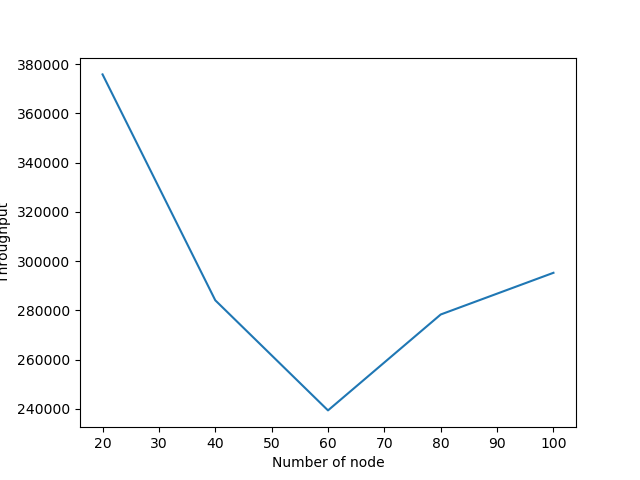
\includegraphics[width=.8\linewidth]{Graph/nodeVsThroughput.png} 
     \caption{Number of Nodes Vs Throughput}
    \label{fig-1}
\end{subfigure}
\begin{subfigure}{.5\textwidth}
  \centering
  % include second image
  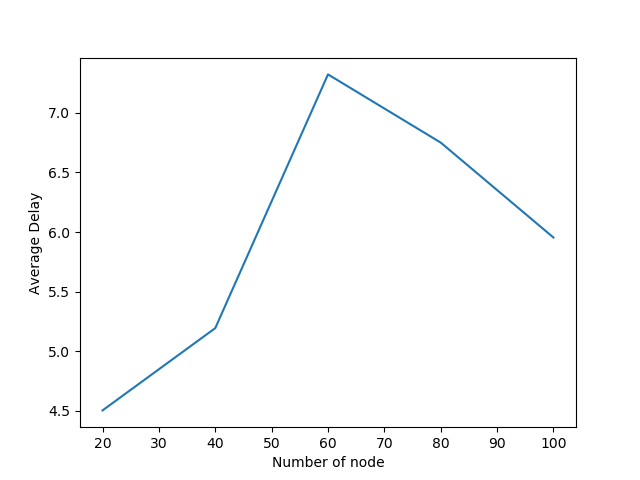
\includegraphics[width=.8\linewidth]{Graph/nodeVsAverageDelay.png} 
    \caption{Number of Nodes Vs Average Delay}
     \label{fig-2}
\end{subfigure}
\begin{subfigure}{.5\textwidth}
  \centering
  % include third image
  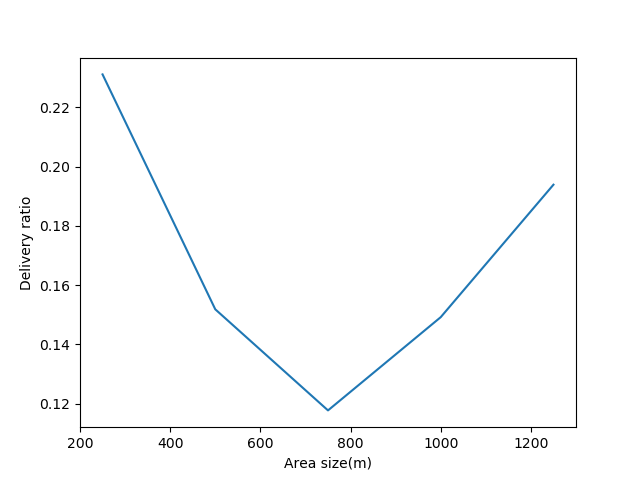
\includegraphics[width=.8\linewidth]{Graph/areaVsDeliveryRatio.png} 
     \caption{Number of Nodes Vs Delivary Ratio}
     \label{fig-3}
\end{subfigure}
\begin{subfigure}{.5\textwidth}
  \centering
  % include fourth image
  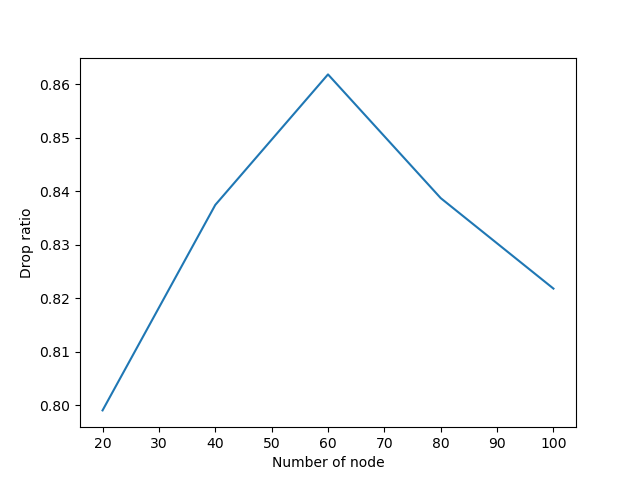
\includegraphics[width=.8\linewidth]{Graph/nodeVsDropRatio.png} 
    \caption{Number of Nodes Vs Drop Ratio}
     \label{fig-4}
\end{subfigure}
\caption{Varying Number of Nodes}
\label{fig:varyingNode}
\end{figure}

\subsection{Varying Number of Flows}
See Figure \ref{fig-5} , \ref{fig-6}, \ref{fig-7} and \ref{fig-8}
\begin{figure}[h]
    \begin{subfigure}{.5\textwidth}
    \centering
    % include first image
    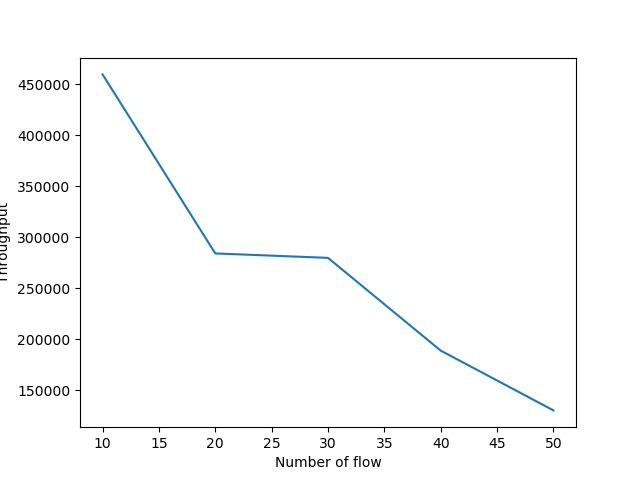
\includegraphics[width=.8\linewidth]{Graph/flowVsThroughput.png}
    \caption{Number of Flows Vs Throughput}
    \label{fig-5}
\end{subfigure}
\begin{subfigure}{.5\textwidth}
    \centering
    % include second image
    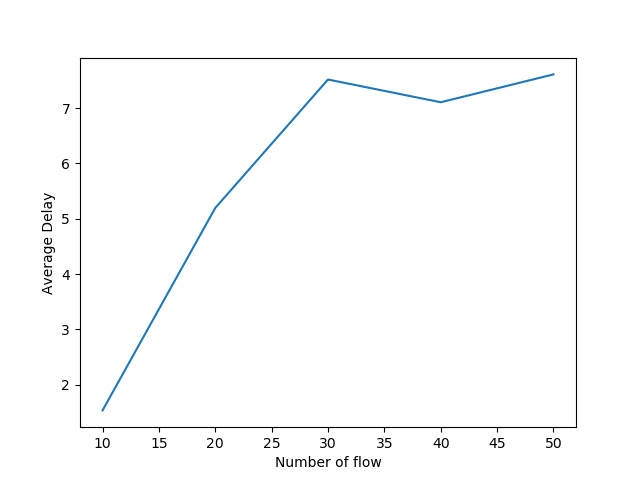
\includegraphics[width=.8\linewidth]{Graph/flowVsAverageDelay.png}
    \caption{Number of Flows Vs Average Delay}
    \label{fig-6}
\end{subfigure}
\begin{subfigure}{.5\textwidth}
    \centering
    % include third image
    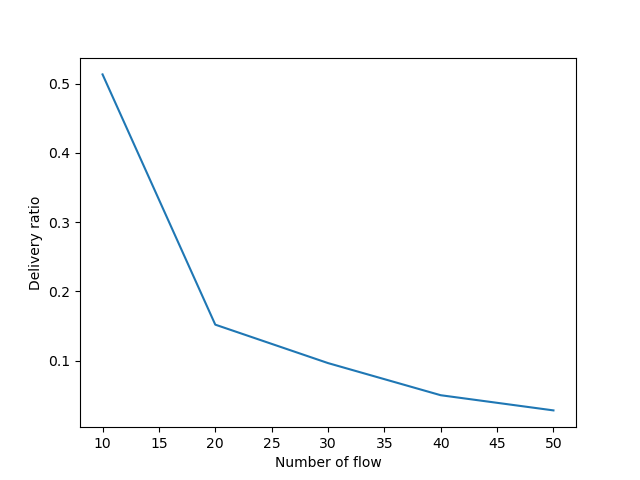
\includegraphics[width=.8\linewidth]{Graph/flowVsDeliveryRatio.png}
    \caption{Number of Flows Vs Delivary Ratio}
    \label{fig-7}
\end{subfigure}
\begin{subfigure}{.5\textwidth}
    \centering
    % include fourth image
    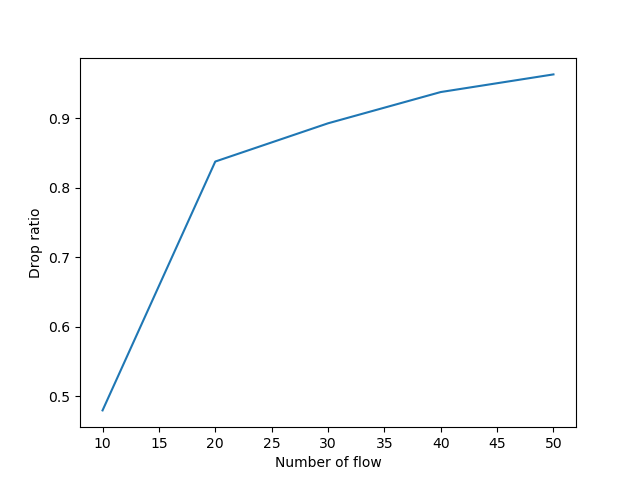
\includegraphics[width=.8\linewidth]{Graph/flowVsDropRatio.png}
    \caption{Number of Flows Vs Drop Ratio}
    \label{fig-8}
\end{subfigure}
\caption{Varying Number of Flows}
\label{fig:varyingFlow}
\end{figure}

\subsection{Varying Area}
See Figure \ref{fig-9} , \ref{fig-10}, \ref{fig-11} and \ref{fig-12}
\begin{figure}[h]
    \begin{subfigure}{.5\textwidth}
    \centering
    % include first image
    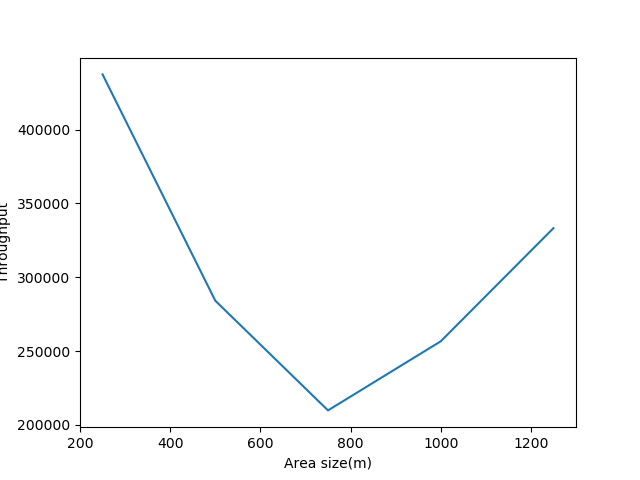
\includegraphics[width=.8\linewidth]{Graph/areaVsThroughput.png}
    \caption{Area Vs Throughput}
    \label{fig-9}
\end{subfigure}
\begin{subfigure}{.5\textwidth}
    \centering
    % include second image
    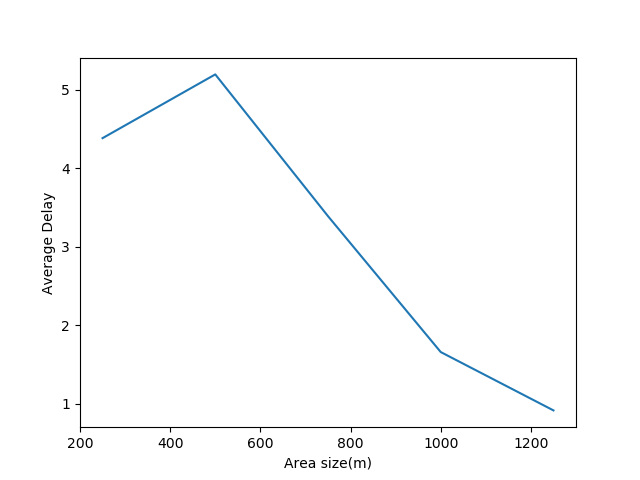
\includegraphics[width=.8\linewidth]{Graph/areaVsAverageDelay.png}
    \caption{Area Vs Average Delay}
    \label{fig-10}
\end{subfigure}
\begin{subfigure}{.5\textwidth}
    \centering
    % include third image
    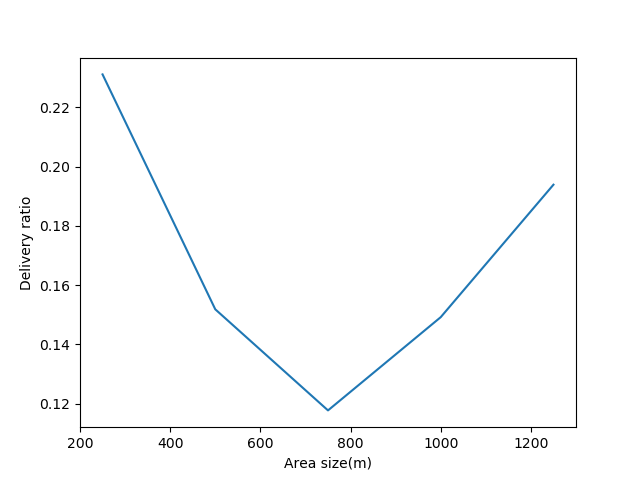
\includegraphics[width=.8\linewidth]{Graph/areaVsDeliveryRatio.png}
    \caption{Area Vs Delivary Ratio}
    \label{fig-11}
\end{subfigure}
\begin{subfigure}{.5\textwidth}
    \centering
    % include fourth image
    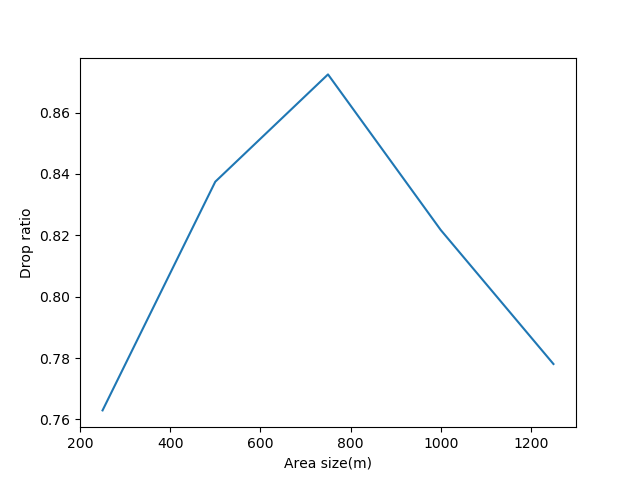
\includegraphics[width=.8\linewidth]{Graph/areaVsDropRatio.png}
    \caption{Area Vs Drop Ratio}
    \label{fig-12}
\end{subfigure}
\caption{Varying Area}
\label{fig:varyingArea}
\end{figure}
\section{Discussion}
\subsection{Varying Number of Node}
This data shows the results of a simulation of a wireless network with a fixed area of 500 and 20 flows, but varying number of nodes, from 20 to 100.

As the number of nodes in the network increases, the drop ratio also increases, indicating that the network becomes more congested and there is a higher likelihood of packets being dropped(See \ref{fig:varyingNode}). The average delay also increases with the number of nodes, reflecting the increased competition for resources in the network. On the other hand, the throughput and delivery ratio both decrease, which suggests that the network becomes less efficient as the number of nodes increases.
\subsection{Varying Number of flow}
This data provides information about the performance of a wireless communication network in a 500 square area with 40 nodes. The number of flows (number of data streams transmitted in parallel) varies from 10 to 50.

The results show that the number of dropped packets increases as the number of flows increases. When the number of flows is 10, the drop ratio is 47.99\% and the delivery ratio is 51.34\%. As the number of flows increases, the drop ratio increases and the delivery ratio decreases. When the number of flows is 50, the drop ratio is 96.27\% and the delivery ratio is only 2.79\%(\ref{fig:varyingFlow}).

Additionally, the average delay and throughput of the network decrease as the number of flows increases. When the number of flows is 10, the average delay is 1.534 seconds and the throughput is 459553 bits/sec. When the number of flows is 50, the average delay is 7.608 seconds and the throughput is 130277 bits/sec.
\subsection{Varying Area}
This data set represents the results of a simulation experiment that studies the impact of the area on network performance. The network has 40 nodes and 20 flows, and the area of the network is varied from 250 to 1250. The key performance metrics considered are throughput, average delay, delivery ratio, and drop ratio.

The results show that as the area of the network increases, the average delay and drop ratio increase, while the throughput and delivery ratio decrease(See \ref{fig:varyingArea}). This can be attributed to the fact that with an increase in the area of the network, the number of hops for a packet to reach its destination increases, which results in increased delay and drop ratio. Furthermore, with an increase in the area, the number of nodes in the network also increases, which results in increased competition for network resources and decreased throughput and delivery ratio.

The data also suggests that the network performance is not uniform for all areas and that there are trade-offs between different performance metrics. For example, in the case of an area of 1250, the network has a higher throughput and delivery ratio compared to other areas, but the average delay is also high. Hence, it is important to consider the specific requirements of a network and make informed decisions while choosing the appropriate network area.

\end{document}
% % \subsection{Varying Area}
% See Figure \ref{fig-9} , \ref{fig-10}, \ref{fig-11} and \ref{fig-12}
% \begin{figure}[h] % [h] forces the figure to be output where it is defined in the code (it suppresses floating)
% 	\centering
% 	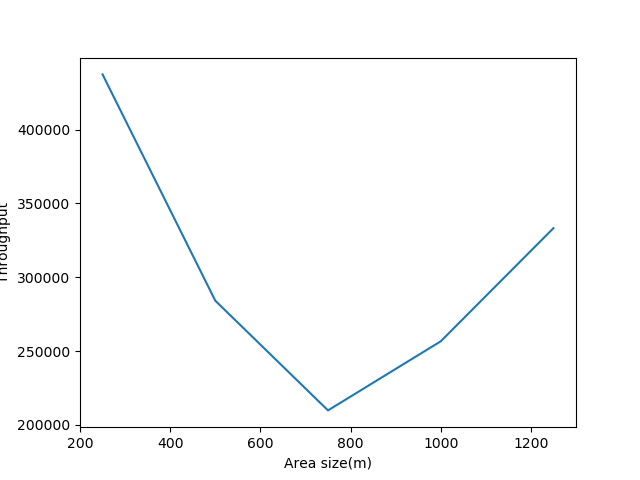
\includegraphics[width=.8\columnwidth]{Graph/areaVsThroughput.png} 
%     \caption{Area Vs Throughput}
%     \label{fig-9}
% \end{figure}
% \begin{figure}[h] % [h] forces the figure to be output where it is defined in the code (it suppresses floating)
% 	\centering
% 	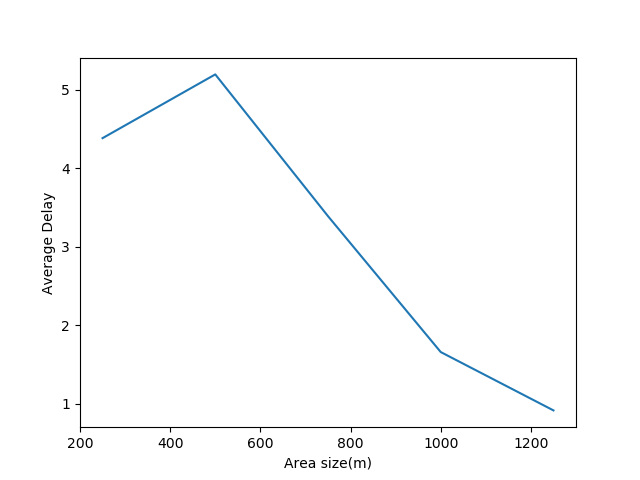
\includegraphics[width=.8\columnwidth]{Graph/areaVsAverageDelay.png} 
%     \caption{Area Vs Average Delay}
%     \label{fig-10}
% \end{figure}
% \begin{figure}[h] % [h] forces the figure to be output where it is defined in the code (it suppresses floating)
%     \centering
%     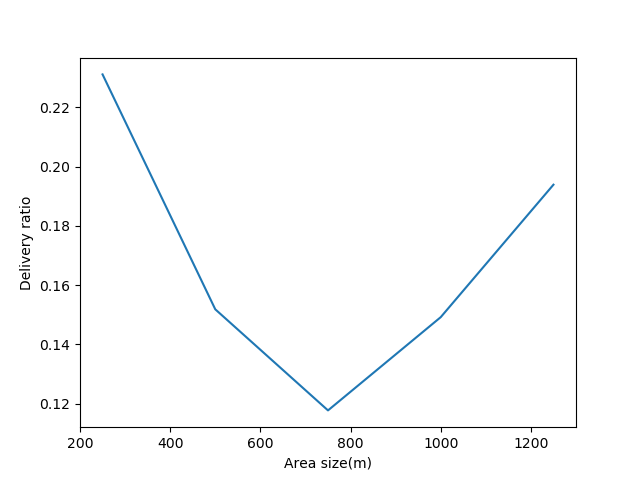
\includegraphics[width=.8\columnwidth]{Graph/areaVsDeliveryRatio.png} 
%     \caption{Area Vs Delivary Ratio}
%     \label{fig-11}
% \end{figure}
% \begin{figure}[h] % [h] forces the figure to be output where it is defined in the code (it suppresses floating)
%     \centering
%     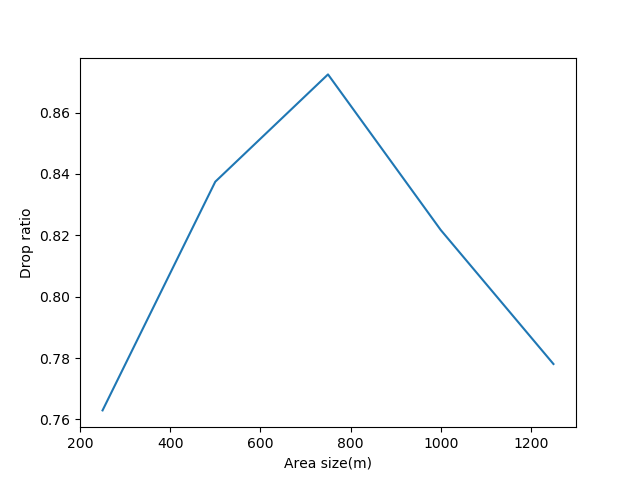
\includegraphics[width=.8\columnwidth]{Graph/areaVsDropRatio.png} 
%     \caption{Area Vs Drop Ratio}
%     \label{fig-12}
% \end{figure}
% \end{document}% % \subsection{Varying Number of Flows}
% % See Figure \ref{fig-5} , \ref{fig-6}, \ref{fig-7} and \ref{fig-8}
% % \begin{figure}[h] % [h] forces the figure to be output where it is defined in the code (it suppresses floating)
% %     \centering
% %     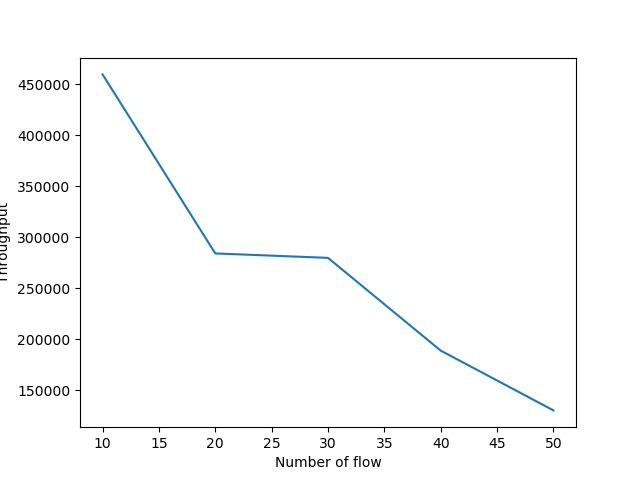
\includegraphics[width=.8\columnwidth]{Graph/flowVsThroughput.png} 
% %     \caption{Number of Flows Vs Throughput}
% %     \label{fig-5}
% % \end{figure}
% % \begin{figure}[h] % [h] forces the figure to be output where it is defined in the code (it suppresses floating)
% %     \centering
% %     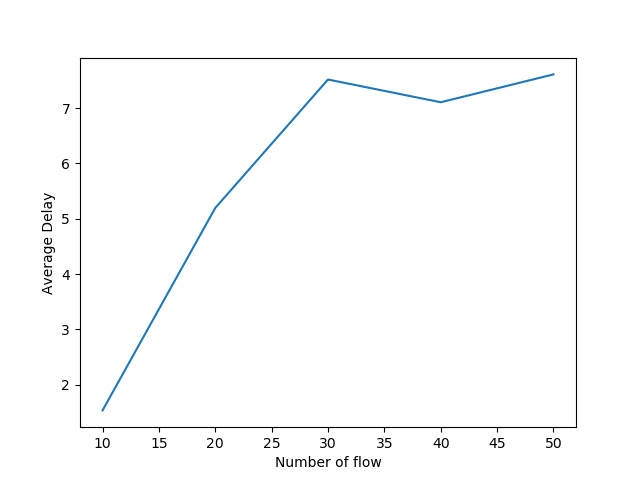
\includegraphics[width=.8\columnwidth]{Graph/flowVsAverageDelay.png} 
% %     \caption{Number of Flows Vs Average Delay}
% %     \label{fig-6}
% % \end{figure}
% % \begin{figure}[h] % [h] forces the figure to be output where it is defined in the code (it suppresses floating)
% %     \centering
% %     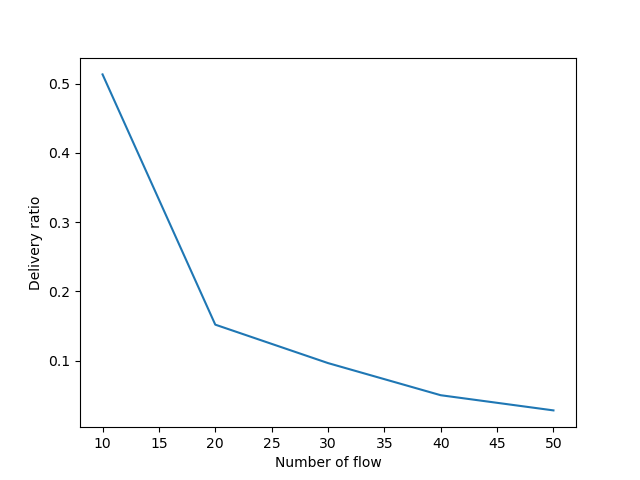
\includegraphics[width=.8\columnwidth]{Graph/flowVsDeliveryRatio.png} 
% %     \caption{Number of Flows Vs Delivary Ratio}
% %     \label{fig-7}
% % \end{figure}
% % \begin{figure}[h] % [h] forces the figure to be output where it is defined in the code (it suppresses floating)
% %     \centering
% %     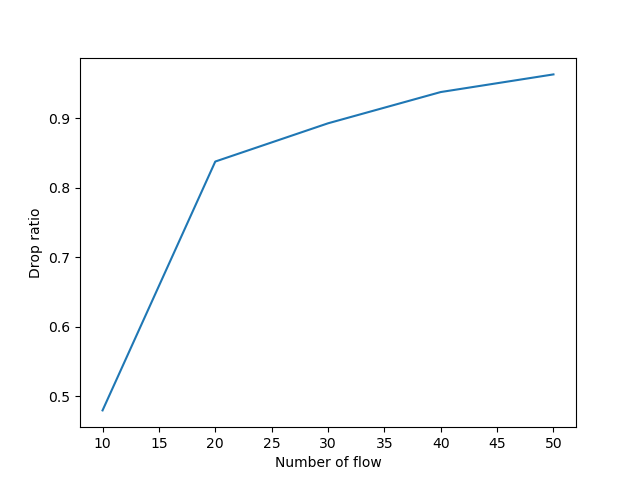
\includegraphics[width=.8\columnwidth]{Graph/flowVsDropRatio.png} 
% %     \caption{Number of Flows Vs Drop Ratio}
% %     \label{fig-8}
% % \end{figure}

% \begin{figure}[h] % [h] forces the figure to be output where it is defined in the code (it suppresses floating)
%     \centering
%     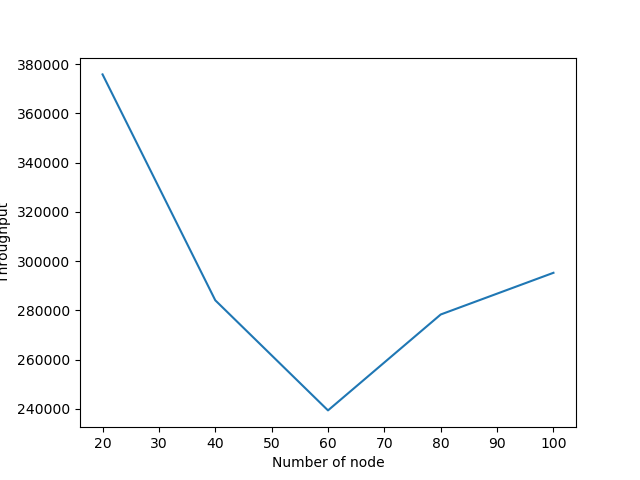
\includegraphics[width=.5\textwidth]{Graph/nodeVsThroughput.png} 
%     \caption{Number of Nodes Vs Throughput}
%     \label{fig-1}
% \end{figure}
% \begin{figure}[h] % [h] forces the figure to be output where it is defined in the code (it suppresses floating)
%     \centering
%     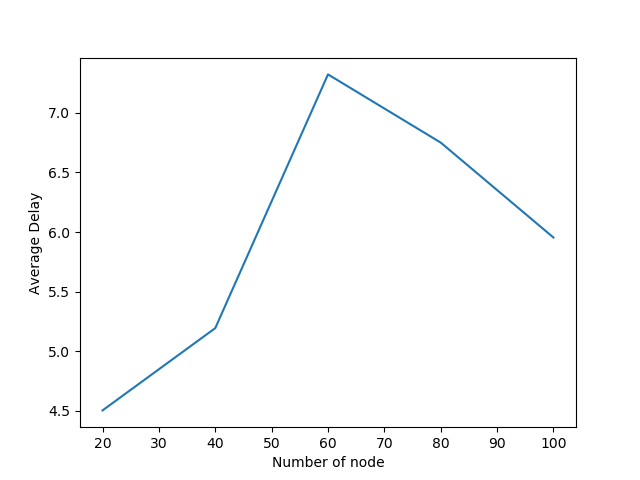
\includegraphics[width=.5\columnwidth]{Graph/nodeVsAverageDelay.png} 
%     \caption{Number of Nodes Vs Average Delay}
%     \label{fig-2}
% \end{figure}
% \begin{figure}[h] % [h] forces the figure to be output where it is defined in the code (it suppresses floating)
%     \centering
%     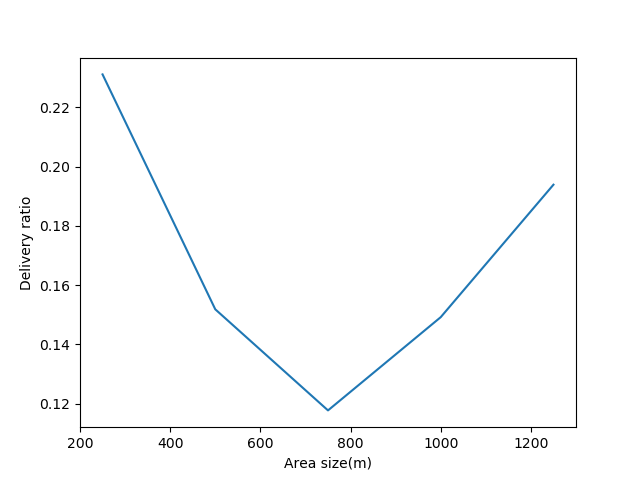
\includegraphics[width=.8\columnwidth]{Graph/areaVsDeliveryRatio.png} 
%     \caption{Number of Nodes Vs Delivary Ratio}
%     \label{fig-3}
% \end{figure}
% \begin{figure}[h] % [h] forces the figure to be output where it is defined in the code (it suppresses floating)
%     \centering
%     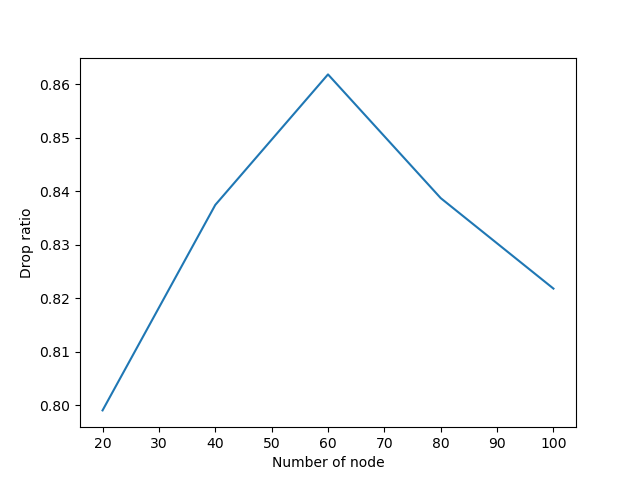
\includegraphics[width=.8\columnwidth]{Graph/nodeVsDropRatio.png} 
%     \caption{Number of Nodes Vs Drop Ratio}
%     \label{fig-4}
% \end{figure}